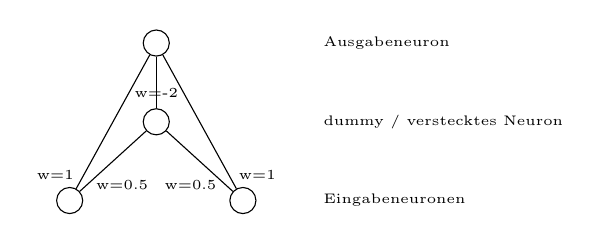
\begin{tikzpicture}[font=\tiny]
	\node (out) at (0,0) [draw,circle]{};
	\node (hidden) at (0,-1) [draw,circle]{};
	\node (in1) at (-1.1,-2) [draw,circle]{};
	\node (in2) at (1.1,-2) [draw,circle]{};

	\draw (out) +(2,0) node[right] {Ausgabeneuron};
	\draw (hidden) +(2,0) node[right] {dummy / verstecktes Neuron};
	\draw (hidden) +(2,-1) node[right] {Eingabeneuronen};

	\draw (in1) -- node[pos=0.1,right]{w=0.5} (hidden);
	\draw (hidden) -- node[pos=0.3]{w=-2} (out);
	\draw (in1) -- node[pos=0.1,left]{w=1}(out);
	\draw (in2) -- node[pos=0.1,left]{w=0.5}(hidden);
	\draw (in2) -- node[pos=0.1,right]{w=1}(out);
\end{tikzpicture}
